% Technical document of team La Espada, More than a Hack 2027 (Phase 1: Ball Possession).
% Typeset with the IEEE conference template (IEEEtran, template version 6/27/2024, ieee.org).
% Build: latexmk -pdf La_Espada.tex   (figures: python solution/reports/figures/make_figures.py)
\documentclass[conference]{IEEEtran}
\IEEEoverridecommandlockouts

\usepackage{cite}
\usepackage{amsmath,amssymb,amsfonts}
\usepackage{graphicx}
\usepackage{textcomp}
\usepackage{xcolor}
\usepackage{booktabs}
\usepackage{tabularx}
\usepackage{url}
\usepackage{balance}
\usepackage{tikz}
\usetikzlibrary{positioning,arrows.meta,calc,fit}
\usepackage[hidelinks]{hyperref}

\graphicspath{{figures/}}
\newcommand{\spf}{spellF1}
\newcommand{\lomo}{LOMO}
\renewcommand{\arraystretch}{1.12}

\begin{document}

\title{Ball Possession from Automatic Tracking:\\ a TCN Ensemble with Event-Gated Decoding}

\author{\IEEEauthorblockN{Team La Espada}
\IEEEauthorblockA{\textit{More than a Hack 2027, Phase 1: Ball Possession} (Metrica Sports $\times$ FC Barcelona)\\
Submitted file \texttt{La\_Espada.csv}, SHA-256 \texttt{8286097e28c9e9ab\ldots888c}\\
Code: \url{https://github.com/MAUK9086/La-Espada-More-than-a-Hack-2027}}}

\maketitle

\begin{abstract}
We label every frame of FC Barcelona v Athletic Club as home possession, away possession or dead ball, using only
the automatic tracking and Smart Tagging of the match. The ranking metric, \spf{}, scores whole possessions, so we
treat the task as temporal segmentation: per-frame evidence for the three states is decoded by a Viterbi pass whose
state changes are cheap only at detected events. The evidence combines hand-written rules on ball--player geometry
with the averaged probabilities of three dilated temporal convolutional networks (TCN). The networks are trained only
on eight external matches, degraded to reproduce the label-free statistics of the provided tracking. In leave-one-match-out evaluation the system reaches \spf{} 0.7590 (0.7077 for our
gradient-boosting predecessor, better on 8 of 8 matches), and 0.7885 and 0.8143 on two held-out matches. Inference
runs in NumPy float64 and regenerates the submitted file byte for byte.
\end{abstract}

\begin{IEEEkeywords}
football analytics, tracking data, ball possession, temporal action segmentation, Viterbi decoding
\end{IEEEkeywords}

\section{Introduction}

The task is to label each of the 199{,}319 frames of the tactical video (25 fps) with \texttt{H} (Barcelona in
possession), \texttt{A} (Athletic Club in possession), \texttt{D} (ball dead) or \texttt{X} (no answer). Two halves,
158{,}857 frames, are graded against a hidden truth derived from corrected tracking. Possession means
\emph{controlled} possession: a touch, a deflection or a lost duel does not change it, and a loose ball stays with the
last team that had it.

\spf{} treats each maximal run of \texttt{H} or of \texttt{A} as one possession, matches predicted and true
possessions one-to-one by temporal intersection-over-union (IoU), and averages the F1 over IoU thresholds 0.3 to 0.7.
Two consequences shape the design. A short flicker of the wrong team splits one possession into two, so a frame
classifier that is right on most frames can still score poorly. Boundaries must also be precise: by the organisers'
example, a perfect labelling shifted by 8 frames scores 0.893.

\section{The Provided Tracking}
\label{sec:data}

The automatic tracking has four defects that every component has to handle.

\emph{Missing ball.} The ball is visible on 59.3\,\% of graded frames. The 150 gaps are long: 85.2\,\% of the
missing frames lie in gaps of 10\,s or more (Fig.~\ref{fig:missing}a). The ball is missing far more often when the
players are slow, which is typical of stoppages (Fig.~\ref{fig:missing}b).

\emph{Smoothed ball with false jumps.} The ball track is heavily smoothed, and 1.8\,\% of consecutive ball positions
imply more than 40\,m/s.

\emph{No player identity.} The 46 track slots hold 2{,}218 tracklets with a median length of 13.6\,s; on 12.9\,\% of
frames one team shows more than 11 objects. Only the team of a slot is reliable.

\begin{figure}[t]
\centering
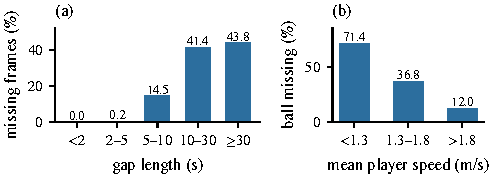
\includegraphics[width=\columnwidth]{fig_missing_ball}
\caption{Missing ball in the provided tracking, label-free statistics. (a) Share of missing frames by gap length
(150 gaps in graded play). (b) Share of frames without a ball by mean player speed; the training degradation
(Section~\ref{sec:degradation}) reproduces these three shares.}
\label{fig:missing}
\end{figure}

\section{Method}

Fig.~\ref{fig:pipeline} summarises the pipeline. Every frame receives a score for each state from two sources, rules
and a learned model, and a Viterbi pass per half selects the best label sequence.

\begin{figure*}[t]
\centering
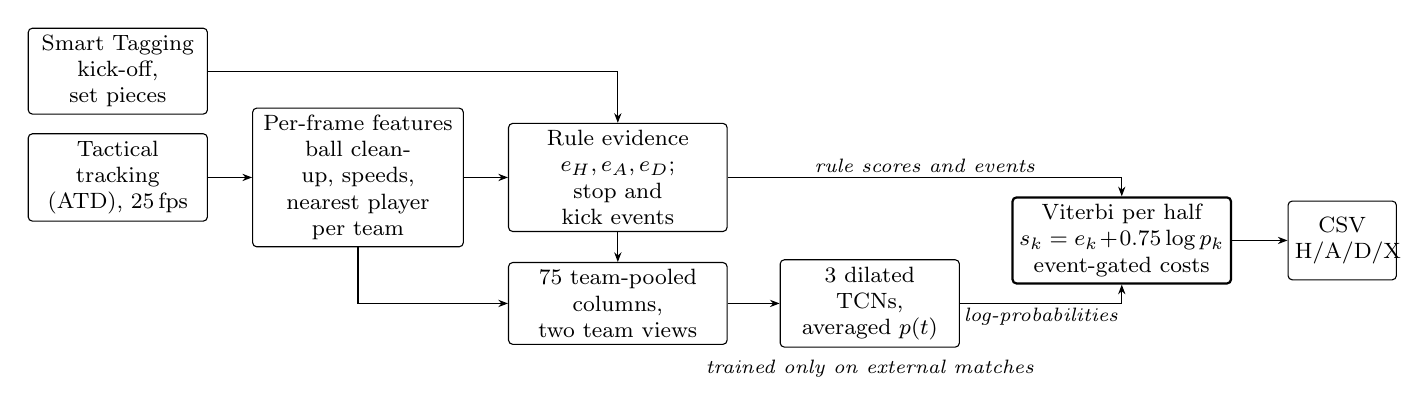
\begin{tikzpicture}[
  font=\footnotesize, >={Stealth[length=3.5pt]},
  box/.style={draw, rounded corners=1.5pt, align=center, inner sep=2.5pt, minimum height=10mm},
  lab/.style={font=\scriptsize\itshape, inner sep=1.5pt}]
  \node[box, text width=21mm] (tag)    at (0,1.35)   {Smart Tagging\\ kick-off, set pieces};
  \node[box, text width=21mm] (atd)    at (0,0)      {Tactical tracking\\ (ATD), 25\,fps};
  \node[box, text width=25mm] (feat)   at (3.05,0)   {Per-frame features\\ ball clean-up, speeds,\\ nearest player per team};
  \node[box, text width=26mm] (rules)  at (6.35,0)   {Rule evidence\\ $e_H, e_A, e_D$;\\ stop and kick events};
  \node[box, text width=26mm] (inputs) at (6.35,-1.6) {75 team-pooled columns,\\ two team views};
  \node[box, text width=21mm] (tcn)    at (9.55,-1.6) {3 dilated TCNs,\\ averaged $p(t)$};
  \node[box, text width=26mm, line width=0.8pt] (vit) at (12.75,-0.8) {Viterbi per half\\ $s_k = e_k + 0.75\log p_k$\\ event-gated costs};
  \node[box, text width=12mm] (out)    at (15.55,-0.8) {CSV\\ H/A/D/X};
  \draw[->] (atd) -- (feat);
  \draw[->] (feat) -- (rules);
  \draw[->] (feat.south) |- (inputs.west);
  \draw[->] (tag.east) -| (rules.north);
  \draw[->] (rules.south) -- (inputs.north);
  \draw[->] (inputs) -- (tcn);
  \draw[->] (rules.east) -| (vit.north);
  \draw[->] (tcn.east) -| (vit.south);
  \draw[->] (vit) -- (out);
  \node[lab, above] at ($(rules.east)!0.5!(rules.east -| vit.north)$) {rule scores and events};
  \node[lab, below] at ($(tcn.east)!0.5!(tcn.east -| vit.south)$) {log-probabilities};
  \node[lab, below=1mm of tcn] {trained only on external matches};
\end{tikzpicture}
\caption{Pipeline. Rule evidence and events (top) and the TCN ensemble (bottom) feed one Viterbi decoder per half.
The rule columns are also inputs of the network. Only the TCNs have trained weights.}
\label{fig:pipeline}
\end{figure*}

\subsection{Per-Frame Features}

Single-frame ball detections that are reached from the previous visible frame \emph{and} left towards the next at
more than 40\,m/s are removed: a genuine fast ball produces one such edge, a false blob two. Ball speed is a centred
difference over $\pm2$ frames. For each team we take the distance $d_k(t)$ from the ball to its nearest player, and
the mean speed $\bar v(t)$ of all tracked players. A ball beyond a line by more than 0.5\,m is \emph{outside}.

\subsection{Rule Evidence}

\emph{Team evidence.} With control radius $R=1.5$\,m, team $k$ gains on frame $t$
\begin{multline}
e_k(t) = u(t)\,\big[\,w(t)\,\mathbf{1}\{d_k\le R,\ d_k<d_{\bar k}\}\\
+ 0.1\,\mathbf{1}\{d_k<d_{\bar k},\ d_k\le 10\,\text{m}\}\big],
\end{multline}
where $u(t)=1$ if the ball is visible and inside the pitch. The weight $w$ is 1 for clear control, 0.3 for a ball
slower than 0.7\,m/s, 0 for a ball faster than 15\,m/s (a ball passing a player is not controlled), at most 0.4 when
an opponent is also within $R$ (a duel), and halved while a restart is pending. The small second term places a switch
inside a ball's flight, near the receiving team.

\emph{Dead-ball evidence.} With slowness $\sigma(t)=\mathrm{clip}\big((2.0-\bar v)/(2.0-1.0),0,1\big)$,
\begin{multline}
e_D = 1.5\,\mathbf{1}_{\text{out}} + 0.4\,\sigma\,\mathbf{1}_{\text{unseen}} + 0.6\,\sigma\,\mathbf{1}_{\text{still}}
+ s_{\text{spot}} + 0.5\,\mathbf{1}_{\text{pending}}\\ + 0.3\,\mathbf{1}_{\text{tag}} - 0.25\,(1-\sigma),
\end{multline}
where $s_{\text{spot}}\in[0.5,1]$ rewards a still ball on a restart spot (the 1.5\,m line band, the goal area, the
centre spot), \emph{pending} marks a ball that crossed a line and has not been struck again (up to 90\,s), and
\emph{tag} marks a Smart Tagging set-piece window before its first strike.

\emph{Events.} A \emph{stop} is the first frame of the ball outside the pitch or the first frame of a tracking gap. A
\emph{kick} is a strike of a still ball: the median ball speed is at most 2.5\,m/s over frames $[t-20,t-5)$, at least
4\,m/s and twice as high over $[t+5,t+15)$, and a player is within 2.5\,m. The windows skip the five frames around
the strike that the tracker's smoothing smears.

\subsection{Learned Evidence: a Dilated TCN Ensemble}
\label{sec:tcn}

\emph{Inputs.} Each frame is described by 75 columns, none of which depends on player identity: per team the centroid,
its forward velocity, width, depth, front and back lines and mean speed; the ball's last known position, signed
velocity, speed and lateral speed, visibility, outside flag and the time since and until it is seen; the gap
between the two team centroids; a simple time-to-intercept pitch control
at the ball; per team the mean distance and forward velocity of the three nearest players and, for the nearest
player, forward velocity, approach speed, speed relative to the ball and goal-side offset; the nearest distances; the
three rule-evidence columns; and for 30 of these a $\pm1$\,s past-versus-future trend. Columns are z-scored with the
training matches' statistics, and missing values are set to 0.

\emph{Team views.} Every match is presented twice: as recorded, and with the teams swapped and the pitch mirrored.
The two predictions are averaged after swapping the \texttt{H} and \texttt{A} outputs of the second, so the model
cannot prefer either team or attacking direction.

\emph{Architecture.} We follow the multi-stage TCN of~\cite{farha2019mstcn} (Fig.~\ref{fig:tcn}). Stage~1 maps
the 75 inputs to 64 channels and applies seven dilated residual blocks ($d=1,2,\dots,64$; receptive field 255
frames, about 10\,s). Stage~2 refines the softmax of stage~1 together with the three rule-evidence columns, with 32
channels and six blocks ($d=1,\dots,32$). A boundary head on stage~1, after ASRF~\cite{ishikawa2021asrf}, predicts
whether a label changes within $\pm2$ frames; it adds a training loss only. Each network has 145{,}991 weights.

\begin{figure}[t]
\centering
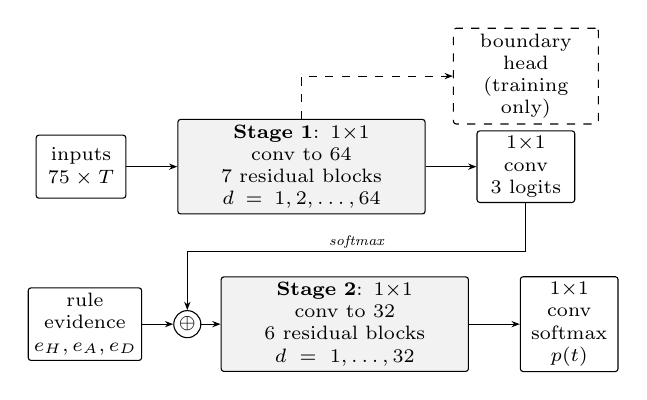
\begin{tikzpicture}[
  font=\scriptsize, >={Stealth[length=3pt]},
  b/.style={draw, rounded corners=1pt, align=center, inner sep=2pt, minimum height=8mm},
  lab/.style={font=\tiny\itshape, inner sep=1pt}]
  \node[b, text width=10mm] (x)  at (0,0)       {inputs\\ $75\times T$};
  \node[b, text width=30mm, fill=black!5] (s1) at (2.8,0) {\textbf{Stage 1}: $1{\times}1$ conv to 64\\ 7 residual blocks\\ $d=1,2,\dots,64$};
  \node[b, text width=11mm] (h1) at (5.65,0)    {$1{\times}1$ conv\\ 3 logits};
  \node[b, text width=17mm, dashed] (bd) at (5.65,1.15) {boundary head\\ (training only)};
  \node[b, text width=13mm] (e)  at (0.05,-2.0) {rule evidence\\ $e_H, e_A, e_D$};
  \node[draw, circle, inner sep=0.6pt] (cat) at (1.35,-2.0) {$\oplus$};
  \node[b, text width=30mm, fill=black!5] (s2) at (3.35,-2.0) {\textbf{Stage 2}: $1{\times}1$ conv to 32\\ 6 residual blocks\\ $d=1,\dots,32$};
  \node[b, text width=11mm] (h2) at (6.2,-2.0)  {$1{\times}1$ conv\\ softmax $p(t)$};
  \draw[->] (x) -- (s1);
  \draw[->] (s1) -- (h1);
  \draw[->, dashed] (s1.north) |- (bd.west);
  \draw[->] (h1.south) -- ++(0,-0.62) coordinate (turn) -| (cat.north);
  \node[lab, above] at ($(turn)!0.5!(turn -| cat.north)$) {softmax};
  \draw[->] (e) -- (cat);
  \draw[->] (cat) -- (s2);
  \draw[->] (s2) -- (h2);
\end{tikzpicture}
\caption{One TCN of the ensemble. A residual block computes
$h \leftarrow h + \mathrm{Drop}_{0.2}\big(W_2\,\mathrm{ReLU}(W_1 *_{d} h)\big)$ with kernel 3 and dilation $d$;
$\oplus$ concatenates channels. The boundary head (dashed) contributes a training loss only.}
\label{fig:tcn}
\end{figure}

\emph{Loss.} For each stage $s$ with log-probabilities $\ell^{s}_{t,c}$ we add the cross-entropy and a truncated
smoothness term~\cite{farha2019mstcn},
\begin{multline}
\mathcal{L} = \sum_{s=1}^{2}\Big[\mathrm{CE}^{s} + \frac{\lambda}{3T}\sum_{t,c}\min\big((\ell^{s}_{t,c}-\ell^{s}_{t-1,c})^2,\tau\big)\Big]\\
+ \mu\,\mathrm{BCE}_{\text{bnd}},
\end{multline}
with $\lambda=0.15$, $\tau=16$, $\mu=0.1$, the gradient stopped through $\ell^{s}_{t-1}$, and the boundary loss
weighted by the ratio of negative to positive frames.

\emph{Ensemble and inference.} Three networks trained with seeds 0, 1 and 2 are averaged. At inference the exported
weights run in NumPy float64 over each whole half (the network is fully convolutional), and the averaged
probabilities are rounded to six decimals before decoding, so floating-point differences between processors cannot
change a label.

\subsection{Decoding}

For state $k\in\{H,A,D\}$ the frame score is $s_k(t)=e_k(t)+\alpha\log\max(p_k(t),10^{-3})$ with $\alpha=0.75$. A
Viterbi pass per half maximises $\sum_t s_{x_t}(t)-\sum_t c(x_{t-1},x_t,t)$ with the costs of
Table~\ref{tab:costs}. A switch between teams costs as much as about 0.3\,s of clear control by the other team; a
stoppage starts cheaply only within three frames of a stop event, and play restarts cheaply only at a kick event. No possession is allowed before each half's
kick-off, detected as the first strike near the centre spot or inside the tagged kick-off window. Frames outside the
graded halves are labelled \texttt{X}.

\begin{table}[t]
\caption{Transition costs of the decoder}
\label{tab:costs}
\centering
\begin{tabular}{@{}lll@{}}
\toprule
change & cost & at an event ($\pm3$ frames)\\
\midrule
\texttt{H}$\leftrightarrow$\texttt{A} & 8 & --\\
live $\to$ \texttt{D} & 15 & 2 at a stop\\
\texttt{D} $\to$ live & 60 & 2 at a kick\\
\bottomrule
\end{tabular}
\end{table}

\section{Training Data, Labels and Degradation}

\subsection{Datasets}

Table~\ref{tab:data} lists every labelled dataset.
The Metrica data is published by Metrica Sports, Sportec Open DFL under CC-BY~4.0, SkillCorner open data under the
MIT licence.

\begin{table}[t]
\caption{Labelled data (all external to the provided match)}
\label{tab:data}
\centering
\footnotesize
\begin{tabularx}{\columnwidth}{@{}>{\raggedright\arraybackslash}X r >{\raggedright\arraybackslash}p{24mm} l@{}}
\toprule
dataset & matches & labels from & use\\
\midrule
Metrica sample data, games 1--2 & 2 & Metrica event data (human coded) & training\\
Metrica sample game 3 & 1 & same & held-out\\
Sportec Open DFL~\cite{bassek2025dfl} (codes in Fig.~\ref{fig:permatch}) & 6 & provider's ball status and possession & training\\
Sportec Open DFL J03WR9 & 1 & same & held-out\\
SkillCorner open data, A-League 2024/25 & 20 & SkillCorner possession annotations & test only\\
\bottomrule
\end{tabularx}
\end{table}

\subsection{Possession Labels}

The external sources mark possession at touch level, so every touch flips it. We convert them to controlled
possession with one mechanical rule: within each live spell the restarting team owns the ball, and possession passes
to the other team only at the start of a run of its own lasting at least 2\,s; shorter runs (touches, deflections,
blocks, lost duels) stay with the current owner, and a stoppage resets the owner. Dead ball comes from the provider's
ball status (DFL) or from the time between a line-crossing or whistle event and the next restart event (Metrica).
The eight training matches hold 2{,}257 possessions under this rule (2{,}845, 2{,}515 and 1{,}870 under 1.0, 1.5 and
3.0\,s rules). No label was added or corrected by hand.

\subsection{Degradation to the Provided Tracking}
\label{sec:degradation}

Each training match is degraded before features are computed:
\begin{itemize}
\item the ball is smoothed with an 8-frame Gaussian and given 2.5\,mm noise, which matches the acceleration
quantiles of the provided ball;
\item each player track drops out in spells (mean visible spell 66\,s, about 93\,\% of players visible);
\item the ball is removed in gaps whose lengths are drawn from the provided match's gap distribution, placed so that
the missing share in each band of mean player speed equals that of the provided tracking (71.4\,\%, 36.8\,\% and
12.0\,\%, Fig.~\ref{fig:missing}b); the band weights are found by iterative correction.
\end{itemize}
We call this the kinematic profile~$k$. It uses only label-free statistics of the provided tracking. Each training
match is used in four independent realisations of the degradation, two of them mirrored across the long axis.

\subsection{Training}

Each network is trained on the eight matches in four realisations and both team views, cut into 60\,s windows (the
last window of a half padded and masked), with Adam (learning rate $5\times10^{-4}$), batch 8, 10 epochs and no early
stopping, on one NVIDIA RTX PRO 4000 GPU with deterministic algorithms. The settings were fixed on leave-one-match-out
results before the held-out matches were scored.

\section{Possession Rules Implemented}

Table~\ref{tab:rules} states where we drew the lines; Section~\ref{sec:robust} measures the effect of the control
rule.

\begin{table}[t]
\caption{Possession rules}
\label{tab:rules}
\centering
\footnotesize
\begin{tabularx}{\columnwidth}{@{}>{\raggedright\arraybackslash}p{23mm}>{\raggedright\arraybackslash}X@{}}
\toprule
situation & rule\\
\midrule
touch, deflection, block, lost duel & no change; a takeover needs a run of at least 2\,s (training labels) and enough evidence to pay the switch cost (decoder)\\
loose ball, ball in flight & stays with the last team until the other team's evidence outweighs the switch cost\\
duel (both teams within 1.5\,m) & weak evidence for the nearer team (0.4)\\
ball tracking gap & possession carried through; dead only with slow players or a line crossing\\
out of play & ball beyond a line by more than 0.5\,m, or a crossing with no strike yet\\
restart & live again only at a strike of a still ball; a throw-in may be struck up to 1.5\,m outside the touchline, and only there\\
kick-off & first strike near the centre spot, or inside the tagged kick-off window\\
foul without a line crossing & from slow players and a still ball, so the stoppage starts late\\
\bottomrule
\end{tabularx}
\end{table}

\begin{figure*}[t]
\centering
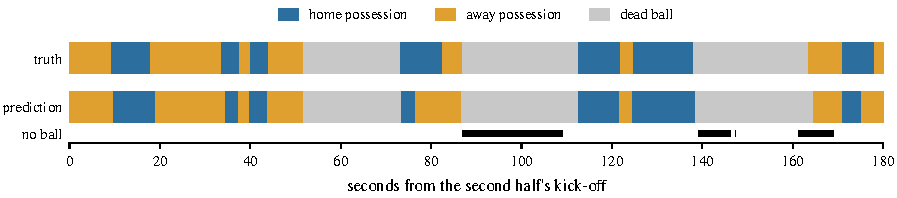
\includegraphics[width=\textwidth]{fig_timeline}
\caption{The first three minutes of the second half of the held-out match DFL J03WR9: true labels, submitted model,
and frames without a ball after degradation. The window was fixed in advance, not selected.}
\label{fig:timeline}
\end{figure*}

\section{Experiments}

\subsection{Protocol}

We use leave-one-match-out (\lomo) over the eight training matches: train on seven, test on the eighth with its
input degraded by profile~$k$. We report the mean \spf{} over the 8 matches and over the 6 DFL matches. Gains are
tested with an exact sign-flip test over matches and a paired bootstrap that resamples possessions within matches
(2{,}000 draws). Two configurations count as different only if their means differ by more than twice the larger of
their between-seed standard deviations. A candidate that passed \lomo{} was then scored once on each held-out match.

\subsection{Main Results}

\begin{table}[t]
\caption{Main results (\spf{}, external matches only)}
\label{tab:main}
\centering
\begin{tabular}{@{}lcc@{}}
\toprule
evaluation & previous & submission\\
\midrule
\lomo, mean of 8 matches & 0.7077 & \textbf{0.7590}\\
\lomo, mean of 6 DFL matches & 0.6889 & \textbf{0.7460}\\
held-out DFL J03WR9 & 0.6895 & \textbf{0.7885}\\
held-out Metrica game 3 & 0.7681 & \textbf{0.8143}\\
\bottomrule
\end{tabular}
\end{table}

Table~\ref{tab:main} compares the submission with our previous version, which used the same rules and decoder but
gradient-boosted trees on frame windows in place of the TCN. The \lomo{} gain is $+0.0513$, positive on all eight
matches (Fig.~\ref{fig:permatch}; sign-flip $p=0.008$), with a bootstrap 5--95\,\% interval of $+0.041$ to $+0.061$.
The three seeds score 0.7518 on average with a between-seed standard deviation of 0.0011; averaging them adds
$+0.0072$. On the held-out matches the macro-F1 is 0.9355 and 0.9211, with 254 and 273 predicted possessions against
267 and 286 true. The gain comes from fewer live frames called dead (2.90\,\% $\to$ 2.14\,\% of graded frames) and
sharper boundaries: the median absolute boundary error of matched possessions falls from 0.41/0.44\,s to 0.23/0.28\,s
(start/end).

\begin{figure}[t]
\centering
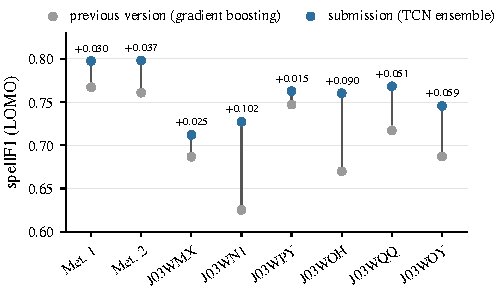
\includegraphics[width=\columnwidth]{fig_per_match}
\caption{\lomo{} \spf{} per training match, previous version and submission; DFL match codes as published.}
\label{fig:permatch}
\end{figure}

\begin{table}[t]
\caption{From rules to the submitted ensemble (\lomo, 8 / 6 DFL)}
\label{tab:steps}
\centering
\footnotesize
\begin{tabularx}{\columnwidth}{@{}>{\raggedright\arraybackslash}X c@{}}
\toprule
system & \spf{}\\
\midrule
rules only, no training & 0.4625 / 0.4278\\
previous version (gradient boosting + refining stage) & 0.7077 / 0.6889\\
TCN, 1 label-placed realisation, 20 epochs (5 seeds) & 0.7301 / 0.7182\\
TCN, 4 realisations of that dropout, 10 epochs (3 seeds) & 0.7443 / 0.7329\\
TCN, 4 realisations of profile $k$ (3 seeds) & 0.7518 / 0.7399\\
\textbf{3-seed ensemble of the row above (submission)} & \textbf{0.7590 / 0.7460}\\
\bottomrule
\end{tabularx}
\end{table}

\subsection{Ablations}

Table~\ref{tab:steps} shows how the recipe was reached. The largest single change is training on several degradation
realisations: four realisations beat one by $+0.017$ at an equal number of training steps. In rows 3--4 the ball
was removed by an earlier profile that placed gaps using each training match's own dead/live labels; profile~$k$
places them by player speed and needs no labels at all.

Changes that did not pass the noise threshold, or lost, were not adopted. Architecture: 128 channels ($-0.0049$),
deeper dilations ($-0.0036$), a third stage ($+0.0003$), a recurrent head ($-0.0093$). Training: label smoothing
($+0.0003$), AdamW with a cosine schedule and weight averaging ($+0.0035$, threshold 0.0093), eight instead of four
realisations ($+0.0007$), an auxiliary touch-level target ($+0.0014$), a per-player set encoder ($-0.0012$).
Decoding: a decoder that forces a 2\,s minimum possession ($+0.0022$, threshold 0.0022), blending with the previous
version ($-0.0012$), test-time mirroring ($+0.0006$).

\subsection{Test on Real Automatic Tracking}

To test transfer beyond simulated degradation we scored 20 SkillCorner matches of broadcast tracking (10\,fps) with
models trained only on our eight matches. All systems score low (0.43--0.48): a different tracker, possession
definition and frame rate. The submission's recipe is $+0.0345$ over the previous version (5--95\,\%: $+0.029$ to
$+0.039$, better on 19 of 20), while the same network trained on the earlier dropout profile is $0.0167$
\emph{below} it; in \lomo{} the two profiles were not separable ($+0.0076$, threshold 0.0087). The difference is
alive/dead: of the true dead frames, the $k$-trained model calls 10.3\,\% live, the previous version 38.5\,\%. This
result decided the training profile. Added as training data, the same matches lowered \lomo{} by 0.040.

\subsection{Sensitivity to the Possession Rule}
\label{sec:robust}

\begin{table}[t]
\caption{\lomo{} \spf{} against truths built with other control rules}
\label{tab:rule}
\centering
\footnotesize
\begin{tabular}{@{}lcccc@{}}
\toprule
trained on & 1.0\,s & 1.5\,s & 2.0\,s & 3.0\,s\\
\midrule
previous version (2\,s) & 0.6385 & 0.6837 & 0.7077 & 0.7067\\
submission (2\,s) & 0.6905 & 0.7357 & \textbf{0.7590} & 0.7469\\
same recipe, 1.5\,s labels & 0.7160 & 0.7511 & 0.7517 & 0.7135\\
\bottomrule
\end{tabular}
\end{table}

The truth's control rule is unknown, so we rebuilt the truth of the eight matches with 1.0 to 3.0\,s rules
(Table~\ref{tab:rule}). The submission beats the previous version under every rule. Training on 1.5\,s labels gives a
better worst case with the same mean (0.7331 against 0.7330) and scored 0.7671 and 0.8176 on the held-out matches
against 0.7885 and 0.8143; with no external evidence for a shorter rule we kept 2\,s.

\subsection{Error Analysis}

Given the true team on every live frame, \lomo{} \spf{} would rise to 0.9367; given the true dead-ball frames, only
to 0.7872. The remaining loss is therefore the team in short exchanges. Possessions of 2--4\,s are 23.7\,\% of true
possessions but 44.4\,\% of the misses (recall 0.52 at IoU 0.5), while above 8\,s the recall is 0.86--0.92.
Fig.~\ref{fig:timeline} shows a typical segment: the segmentation follows the truth, and the errors are switches
placed a few seconds early or late. On corrected tracking the recipe reaches 0.8217, and with a never-missing ball
0.7903 (0.7523 on degraded input, same seed).

\subsection{Provided Match}

Without labels, the submission predicts 261 possessions, 120 stoppages and 45.4\,\% dead frames; 5.22\,\% of graded
frames differ from the previous version. The public five minutes were scored only after the decision, as a pipeline
check: \spf{} 0.6353 and macro-F1 0.8433, against 0.6941 and 0.7775 for the previous version, both with 17 predicted
possessions against 17 true. It played no part in any choice.

\begin{table}[t]
\caption{Assets of the provided match: used and dropped}
\label{tab:assets}
\centering
\footnotesize
\begin{tabularx}{\columnwidth}{@{}>{\raggedright\arraybackslash}p{20mm} l >{\raggedright\arraybackslash}X@{}}
\toprule
asset & & how and why\\
\midrule
tactical tracking & used & the only tracking input\\
Smart Tagging & used & kick-off windows; a small dead-ball term in set-piece windows (automatic output)\\
half boundaries & used & graded frames; \texttt{X} outside them\\
tactical video & dropped & a pretrained ball detector's candidates were mostly far from the tracked ball; a ball that is never missing would add only $+0.038$\\
broadcast assets & dropped & own timeline, no external data to validate a fusion\\
public 5 minutes & check & scored after each decision, never used to choose or tune\\
\bottomrule
\end{tabularx}
\end{table}

\section{Rules Compliance}
\label{sec:compliance}

Table~\ref{tab:assets} lists the assets of the provided match we used and dropped. Training, tuning and every
selection used external data only; the provided tracking and Smart Tagging are model input
only. No hand labels or corrections, no frame-specific rules or constants, no check against the video. We state three
points openly. (i) The degradation of the external matches reproduces label-free statistics of the provided tracking:
the ball's missing share, gap lengths, missing share by player speed and acceleration. (ii) Four logic errors in the
rule evidence were noticed while inspecting the public window (e.g.\ a ball carried back over the goal line was
treated as a restart); each was fixed with a general rule and checked on external matches. (iii) An early version
simulated ball dropout with rates read from public-window labels; it was replaced by the label-free profile~$k$.

\section{Limitations and Future Work}

All scores come from external matches with simulated degradation; on the only real-tracker test every system scored
below 0.5, so transfer to the provided tracker is the main uncertainty. The truth's control rule is unknown (half a
second costs up to 0.02). Possessions under 4\,s cause half of the misses, fouls without a line crossing are detected
late, and the Smart Tagging path is unvalidated (no external match has tags). The evidence base is small: eight
training matches, two held-out matches used for several candidates. Next we would add labelled matches with
corrected tracking, learn a control model for contested balls, and calibrate the degradation on a second tracker.

\section{Reproduction}

{\raggedright
With Python 3.13, the pinned \texttt{solution/\allowbreak requirements.txt} (no GPU needed) and the organisers'
bundle in \texttt{data/}, \texttt{python solution/run.py} writes \texttt{La\_Espada.csv} (SHA-256
\texttt{8286097e\ldots}) and validates it in 30--100\,s. Retraining commands are in the README.\par}

\bibliographystyle{IEEEtran}
\begin{thebibliography}{1}

\bibitem{farha2019mstcn}
Y.~Abu~Farha and J.~Gall, ``MS-TCN: Multi-stage temporal convolutional network for action segmentation,'' in
\emph{Proc. IEEE/CVF Conf. Computer Vision and Pattern Recognition (CVPR)}, 2019, pp.~3575--3584.

\bibitem{ishikawa2021asrf}
Y.~Ishikawa, S.~Kasai, Y.~Aoki, and H.~Kataoka, ``Alleviating over-segmentation errors by detecting action
boundaries,'' in \emph{Proc. IEEE/CVF Winter Conf. Applications of Computer Vision (WACV)}, 2021, pp.~2322--2331.

\bibitem{bassek2025dfl}
M.~Bassek, R.~Rein, H.~Weber, and D.~Memmert, ``An integrated dataset of spatiotemporal and event data in elite
soccer,'' \emph{Scientific Data}, vol.~12, 2025, doi: 10.1038/s41597-025-04505-y.

\end{thebibliography}

\end{document}
